\حصہ{دیگر شرح تبدیلی}
ٹینکی سے \عددی{\SI{3000}{\liter\per\minute}} پانی کے انعکاس سے ٹینکی میں پانی کی گہرائی کس شرح سے تبدیل ہو گی؟ اس طرح کے سوالات میں ہم اس شرح کو معلوم کرنا چاہتے  ہیں جس کو ہم ناپ نہیں سکتے ہیں۔قابل ناپ شرح استعمال کرتے ہوئے یہ معلومات حاصل کی جاتی ہے۔

\ابتدا{مثال}\شناخت{مثال_تفرق_انعکاس}\ترچھا{انعکاس}\\
\عددی{\SI{3000}{\liter\per\minute}} کی شرح سے انعکاس کی صورت میں ٹینکی میں پانی کی گہرائی کم ہونے کی شرح جاننے کی خاطر ہم رداس \عددی{r} کی ٹینکی لیتے ہیں جس میں پانی کی گہرائی \عددی{h} ہے۔یوں پانی کا حجم \عددی{H=\pi r^2h} ہو گا جہاں حجم کو \عددی{H} سے ظاہر کیا گیا ہے (شکل \حوالہ{شکل_مثال_تفرق_انعکاس})۔اب ہمیں انعکاس
\begin{align*}
\frac{\dif H}{\dif t}=-3000
\end{align*}
بتلایا گیا ہے جہاں \عددی{t} وقت کو ظاہر کرتی ہے اور وقت کے ساتھ حجم کم ہونے کو منفی کی علامت سے ظاہر کیا گیا ہے۔ہمیں
\begin{align*}
\frac{\dif h}{\dif t}
\end{align*}
تلاش کرنا ہے۔ایسا کرنے کی خاطر ہمیں \عددی{H} اور \عددی{h} کا تعلق مساوات کی صورت میں لکھنا ہو گا۔یہ مساوات متغیرات کی اکائیوں پر منحصر ہو گی۔یوں حجم کو لٹر جبکہ رداس اور گہرائی کو میٹر میں رکھتے ہوئے درج ذیل لکھا جا سکتا ہے۔
\begin{align*}
H=1000\pi r^2h
\end{align*}
یاد رہے کہ ایک  مربع میٹر میں \عددی{1000} لٹر ہوتے ہیں۔دونوں اطراف کا وقت کے ساتھ تفرق لیتے ہیں
\begin{align*}
\frac{\dif H}{\dif t}=1000\pi r^2\frac{\dif h}{\dif t}
\end{align*}
جہاں دائیں جانب \عددی{r} مستقل ہے۔اس میں \عددی{\tfrac{\dif H}{\dif t}} کی معلوم قیمت پر کرتے ہوئے نا معلوم شرح \عددی{\tfrac{\dif h}{\dif t}} حاصل کرتے ہیں۔
\begin{align*}
\frac{\dif h}{\dif t}=\frac{-3000}{1000\pi r^2}=-\frac{3}{\pi r^2}
\end{align*}
پانی کی گہرائی \عددی{\tfrac{3}{\pi r^2}} میٹر فی منٹ کی شرح سے کم ہو گی۔آپ دیکھ سکتے ہیں کہ یہ شرح رداس پر منحصر ہے۔ کم رداس کی صورت میں شرح زیادہ اور زیادہ رداس کی صورت میں شرح کم ہو گی۔مثلاً \عددی{r=\SI{1}{\meter}} اور \عددی{r=\SI{10}{\meter}} کی صورت میں شرح درج ذیل ہوں گی۔
\begin{align*}
\frac{\dif h}{\dif t}&=-\frac{3}{\pi}\approx \SI{-0.95}{\meter\per\minute}=\SI{-95}{\centi\meter\per\minute}&&(r=\SI{1}{\meter})\\
\frac{\dif h}{\dif t}&=-\frac{3}{100\pi}\approx \SI{-0.0095}{\meter\per\minute}=\SI{-0.95}{\centi\meter\per\minute}&&(r=\SI{10}{\meter})
\end{align*}
%
\begin{figure}
\centering
\begin{minipage}{0.45\textwidth}
\centering
\begin{tikzpicture}
\draw(0,2.25) circle (1cm and 0.25cm);
\draw([shift={(0:1cm and 0.25cm)}]0,0) arc (0:-180:1cm and 0.25cm);
\draw(-1,0)--(-1,2.25);
\draw(1,0)--(1,2.25);
\draw([shift={(0:1cm and 0.25cm)}]0,1.5) arc (0:-180:1cm and 0.25cm);
\draw[gray]([shift={(0:1cm and 0.25cm)}]0,1.5) arc (0:180:1cm and 0.25cm);
\draw[stealth-stealth] (1.25,0)--(1.25,1.5)node[pos=0.5,right]{$h$};
\draw[-stealth](-1.25,1.5)--(-1.25,1)node[pos=0.5,left]{$\tfrac{\dif h}{\dif t}=?$};
\fill[white](-1.25,0) rectangle++(0.5,0.25);
\draw(-1,0.25)--++(-0.25-0.25,0)--++(0,-0.25-0.25)coordinate(kA);
\draw(-1,0)--++(-0.25,0)--++(0,-0.25)coordinate(kB);
\draw(-1,0) to [out=70,in=-70] (-1,0.25);
\draw(kA) to [out=-20,in=-160] (kB);
\draw[-stealth](kA)++(0.125,-0.1)--++(0,-0.5)node[pos=0.5,right]{$\tfrac{\dif H}{\dif t}=\SI{-3000}{\litre\per\minute}$};
\end{tikzpicture}
\caption{پانی کی ٹینکی (مثال \حوالہ{مثال_تفرق_انعکاس})}
\label{شکل_مثال_تفرق_انعکاس}
\end{minipage}\hfill
\begin{minipage}{0.45\textwidth}
\centering
\begin{tikzpicture}
\pgfmathsetmacro{\ang}{atan(2/3)}
\pgfmathsetmacro{\r}{0.4}
\draw[fill=lgray](0,0) circle (\r);
\draw(-\r,-0.1)--++(0.25,-0.75)coordinate(kA);
\draw(\r,-0.1)--++(-0.25,-0.75);
\draw[fill=lgray](kA)--++(0.3,0)--++(0,-0.15)--++(-0.3,0)--++(0,0.15);
\draw(kA)++(0.15,-0.15)coordinate(kB)--++(0,-2)node[pos=0.5,right]{$y$}--++(-3,0)coordinate(kC)node[pos=0.5,below]{$\SI{100}{\meter}$}node[circ]{}node[left]{\RL{فاصلہ پیما}}--(kB);
\draw[-stealth](kB)++(0.5,0)--++(0,0.25)node[pos=0.5,right]{$\tfrac{\dif y}{\dif t}=?$};
\draw[-stealth]([shift={(0:0.5)}]kC) arc (0:\ang:0.5);
\draw(kC)++(\ang/2:0.8)node[]{$\theta$};
\end{tikzpicture}
\caption{غبارہ (مثال \حوالہ{مثال_تفرق_غبارہ})}
\label{شکل_مثال_تفرق_غبارہ}
\end{minipage}
\end{figure}
\انتہا{مثال}
%=======================
\ابتدا{مثال}\شناخت{مثال_تفرق_غبارہ}\ترچھا{غبارہ کی اڑان}
گرم ہوا کا غبارہ زمین سے سیدھا آسمان کی طرف اٹھتا ہے (شکل \حوالہ{شکل_مثال_تفرق_غبارہ})۔ غبارے کی نقطہ اڑان  سے \عددی{\SI{100}{\meter}}  دور واقع \ترچھا{فاصلہ  پیما}\فرہنگ{پیما!فاصلہ}\حاشیہب{range finder}\فرہنگ{range finder} سے غبارے پر نظر رکھی جاتی ہے۔جس لمحہ فاصلہ پیما کا زاویہ صعود \عددی{\tfrac{\pi}{4}} تھا اس لمحہ زاویہ کی تبدیلی کی شرح \عددی{\SI{0.14}{\radian\per\minute}} تھی۔اس لمحہ پر غبارہ کس رفتار سے اوپر جا رہا تھا؟\\
حل:\quad
ہم اس کا جواب چھ قدموں میں دیتے ہیں۔\\
\موٹا{پہلا قدم:}\quad 
موقع کی تصور کشی کریں اور متغیرات کی نشاندہی کریں۔تصویر میں متغیرات \عددی{\theta} اور \عددی{y} درج ذیل ہیں جو بالترتیب فاصلہ پیما کا زاویہ صعود اور غبارے کی بلندی کو ظاہر کرتے ہیں۔ہم وقت کو \عددی{t} سے ظاہر کرتے ہیں اور فرض کرتے ہیں کہ \عددی{\theta} اور \عددی{y} متغیر \عددی{t} کے قابل تفرق تفاعل ہیں۔فاصلہ پیما سے غبارے کے ابتدائی مقام تک فاصلہ \عددی{\SI{100}{\meter}} ہے جس کر متغیر سے ظاہر کرنے کی ضرورت نہیں ہے۔\\
\موٹا{دوسرا قدم:}\quad
ان معلومات کو الجبرائی روپ میں لکھتے ہیں۔
\begin{align*}
\frac{\dif \theta}{\dif t}=\SI{0.14}{\radian\per\minute}&& (\theta=\tfrac{\pi}{4})
\end{align*}
\موٹا{تیسرا قدم:} \quad
جو ہم سے پوچھا گیا ہے اس کو لکھیں۔ہم سے \عددی{\theta=\pi/4} کی صورت میں \عددی{\tfrac{\dif y}{\dif t}} پوچھا گیا ہے۔\\
\موٹا{چوتھا قدم:}\quad
متغیرات  \عددی{\theta} اور \عددی{y} کا آپس میں تعلق لکھیں۔
\begin{align*}
\frac{y}{100}=\tan\theta\quad \implies \quad y=100\tan\theta
\end{align*}
\موٹا{پانچواں قدم:}\quad
زنجیری قاعدہ استعمال کرتے ہوئے \عددی{t} کے لحاظ سے تفرق حاصل کریں جو \عددی{\tfrac{\dif y}{\dif t}} (درکار معلومات) اور \عددی{\tfrac{\dif \theta}{\dif t}} (معلوم معلومات)  کے بیچ تعلق دیگا۔
\begin{align*}
\frac{\dif y}{\dif t}=100\sec^2\theta\frac{\dif \theta}{\dif t}
\end{align*}
\موٹا{چھٹا قدم:}\quad
\عددی{\theta=\tfrac{\pi}{4}} اور \عددی{\tfrac{\dif \theta}{\dif t}=0.14} پر کرتے ہوئے \عددی{\tfrac{\dif y}{\dif t}} کی قیمت تلاش کریں۔
\begin{align*}
\frac{\dif y}{\dif t}=100(\sec\tfrac{\pi}{4})^2(0.14)=\SI{28}{\meter\per\minute}
\end{align*}
\انتہا{مثال}
%========================

\موٹا{اس طرح کے مسائل حل کرنے کا لائحہ عمل}
\begin{itemize}

\item
مسئلے کی تصور کشی کریں۔وقت کو \عددی{t} سے ظاہر کریں اور تمام متغیرات کو \عددی{t} کے قابل تفرق تفاعل تصور کریں۔
\item
اعدادی معلومات کو منتخب کردہ متغیرات کی روپ میں لکھیں۔
\item
مطلوبہ شرح یا متغیر کو لکھیں (جو شرح کی صورت میں عموماً تفرق کی روپ میں ہو گا)۔
\item
متغیرات کا آپس میں تعلق لکھیں۔کئی بار آپ کو دو یا دو سے زیادہ مساواتوں کو اکٹھے کرتے ہوئے ایک مساوات حاصل کرنا ہو گا۔
\item
اس کا \عددی{t} کے لحاظ سے تفرق لیں۔اس کے بعد درکار شرح کو باقی متغیرات (جن کی قیمتیں آپ جانتے ہیں) کی صورت میں لکھیں۔
\item
معلوم معلومات کو پر کرتے ہوئے نا معلوم شرح کی قیمت دریافت کریں۔
\end{itemize}


%
\ابتدا{مثال}
پولیس ایک گاڑی کا پیچھا کر رہی ہے۔ جب چوک سے پولیس کی گاڑی کا فاصلہ \عددی{\SI{0.6}{\kilo\meter}} اور  بھاگنے والی گاڑی کا فاصلہ \عددی{\SI{0.8}{\kilo\meter}} ہے  اس لمحہ پر دونوں گاڑیوں کے بیچ فاصلہ \عددی{\SI{20}{\kilo\meter\per\hour}} سے بڑھ رہا ہے۔پولیس کی گاڑی کی رفتار \عددی{\SI{60}{\kilo\meter\per\hour}} ہونے کی صورت میں بھاگنے والی گاڑی کی رفتار کیا ہو گی؟\\
حل:\quad
ہم مذکورہ بالا اقدام پر چلتے ہوئے مسئلے کو حل کرتے ہیں۔\\
\موٹا{پہلا قدم:}\quad
\ترچھا{تصویر اور متغیرات۔} ہم کارتیسی محدد پر تصویر کشی کرتے ہیں۔ چوک کو مبدا پر رکھتے ہوئے بھاگنے والی گاڑی کو \عددی{x} محور جبکہ پولیس کی گاڑی کو \عددی{y} محور پر رکھتے ہیں۔ وقت کو \عددی{t} سے ظاہر کرتے ہوئے لمحہ \عددی{t} پر بھاگنے والی گاڑی کا مقام \عددی{x}, پولیس کی گاڑی کا مقام \عددی{y} اور دونوں گاڑیوں کے بیچ فاصلہ \عددی{s} ہے۔ ہم فرض کرتے ہیں کہ \عددی{x}، \عددی{y} اور \عددی{s} متغیر \عددی{t} کے قابل تفرق تفاعل ہیں۔\\
\موٹا{دوسرا قدم:}\quad
\ترچھا{اعدادی معلومات۔} لمحہ \عددی{t} پر درج ذیل ہمیں معلوم ہے۔
\begin{align*}
x=\SI{0.8}{\kilo\meter},\quad y=\SI{0.6}{\kilo\meter},\quad \frac{\dif y}{\dif t}=\SI{-60}{\kilo\meter\per\hour},\quad \frac{\dif s}{\dif t}=\SI{20}{\kilo\meter\per\hour}
\end{align*}  
\عددی{\tfrac{\dif y}{\dif t}} اس لئے منفی ہے کہ پولیس کی گاڑی مبدا کی طرف یعنی گھٹتی \عددی{y}  رخ چل رہی ہے۔\\
\موٹا{تیسرا قدم:}\quad
ہمیں \عددی{\tfrac{\dif x}{\dif t}} تلاش کرنا ہے۔\\
\موٹا{چوتھا قدم:}\quad
مسئلہ فیثاغورث کے تحت متغیرات کا تعلق \عددی{s^2=x^2+y^2} ہے۔\\
\موٹا{پانچواں قدم:}\quad
زنجیری قاعدہ کی مدد سے \عددی{t} کے لحاظ سے تفرق لیتے ہیں۔
\begin{align*}
2s\frac{\dif s}{\dif t}&=2x\frac{\dif x}{\dif t}+2y\frac{\dif y}{\dif t}\\
\frac{\dif s}{\dif t}&=\frac{1}{s}\big(x\frac{\dif x}{\dif t}+y\frac{\dif y}{\dif t}\big)\\
&=\frac{1}{\sqrt{x^2+y^2}}\big(x\frac{\dif x}{\dif t}+y\frac{\dif y}{\dif t}\big)
\end{align*}
\موٹا{چھٹا قدم:}\quad
\عددی{x=0.8}، \عددی{y=0.6}، \عددی{\tfrac{\dif y}{\dif t}=-60} اور \عددی{\tfrac{\dif s}{\dif t}=20} پر کرتے ہوئے \عددی{\tfrac{\dif x}{\dif t}} کی قیمت معلوم کریں۔
\begin{align*}
20&=\frac{1}{\sqrt{0.8^2+0.6^2}}\big(0.8\frac{\dif x}{\dif t}+0.6(-60)\big)\\
20&=0.8\frac{\dif x}{\dif t}-36\\
\frac{\dif x}{\dif t}&=\frac{20+36}{0.8}=70
\end{align*}
اس لمحہ پر بھاگنے والی گاڑی کی رفتار \عددی{\SI{70}{\kilo\meter\per\hour}} ہے۔ 

\انتہا{مثال}
%==================
\ابتدا{مثال}
پانی کی مخروطی ٹینکی  \عددی{\SI{9}{\meter\cubed\per\minute}} شرح سے بھری جاتی ہے۔مخروط کے قاعدہ کا رداس \عددی{\SI{5}{\meter}}، اس کا قد \عددی{\SI{10}{\meter}} ہے  اور اس کی نوک نیچے جانب ہے۔جس لمحہ پانی کی گہرائی \عددی{\SI{6}{\meter}} ہو اس لمحہ گہرائی کس شرح سے بڑھتی ہے؟\\
حل:\quad
ہم مذکورہ بالا اقدام پر چلتے ہوئے اس مسئلہ کو حل کرتے ہیں۔\\
\موٹا{پہلا قدم:}\quad
\ترچھا{تصویر کشی اور متغیرات۔} نیم بھری ٹینکی کی شکل بناتے ہیں۔اس مسئلے کے متغیرات درج ذیل ہیں۔
\begin{description}
\item[$:H$]
لمحہ \عددی{t} (منٹ) پر ٹینکی میں پانی کا حجم (مربع میٹر)۔
\item[$:x$]
لمحہ \عددی{t} (منٹ) پر پانی کی سطح کا رداس (میٹر)۔
\item[$:y$]
لمحہ \عددی{t} (منٹ) پر پانی کی گہرائی (میٹر)۔
\end{description}
ہم فرض کرتے ہیں کہ \عددی{H}، \عددی{x} اور \عددی{y} متغیر \عددی{t} کے قابل تفرق تفاعل ہیں۔ٹینکی کی جسامت مستقل مقدار ہے۔\\
\موٹا{دوسرا قدم:}\quad
\ترچھا{اعدادی معلومات۔} لمحہ \عددی{t} پر ہمیں درج ذیل معلوم ہے۔
\begin{align*}
y=\SI{6}{\meter},\quad \frac{\dif H}{\dif t}=\SI{9}{\meter\cubed\per\minute}
\end{align*}
\موٹا{تیسرا قدم:}\quad
\ترچھا{ہمیں} \عددی{\tfrac{\dif y}{\dif t}} \ترچھا{تلاش کرنا ہے۔}\\
\موٹا{چوتھا قدم:}\quad
متغیرات کا آپس میں تعلق:
\begin{align*}
H=\frac{1}{3}\pi x^2 y
\end{align*}
چونکہ لمحہ \عددی{t} پر ہمیں \عددی{x} اور \عددی{\tfrac{\dif x}{\dif t}} کے بارے میں معلومات فراہم نہیں کی گئی ہے لہٰذا ہمیں \عددی{x} سے چھٹکارا حاصل کرنا ہو گا۔ متشابہ مثلثات استعمال کرتے ہوئے شکل سے
\begin{align*}
\frac{x}{y}=\frac{5}{10}\quad \implies \quad x=\frac{y}{2}
\end{align*}
لکھا جا سکتا ہے۔یوں درج ذیل ہو گا۔
\begin{align*}
H=\frac{1}{3}\pi (\tfrac{y}{2})^2y=\frac{\pi}{12}y^3
\end{align*}
\موٹا{پانچواں قدم:}\quad
\عددی{t} \ترچھا{کے لحاظ سے تفرق۔} درج بالا مساوات کا تفرق لیتے ہیں۔
\begin{align*}
\frac{\dif H}{\dif t}=\frac{\pi}{12} \cdot 3y^2\frac{\dif y}{\dif t}=\frac{\pi}{4}y^2\frac{\dif y}{\dif t}
\end{align*}
اس کو \عددی{\tfrac{\dif y}{\dif t}} کے لئے حل کرتے ہیں۔
\begin{align*}
\frac{\dif y}{\dif t}=\frac{4}{\pi y^2}\frac{\dif H}{\dif t}
\end{align*}
\موٹا{چھٹا قدم:}\quad
\ترچھا{دی گئی معلومات  یعنی}  \عددی{y=6} اور \عددی{\tfrac{\dif H}{\dif t}=9} پر کرتے ہیں۔
\begin{align*}
\frac{\dif y}{\dif t}=\frac{4}{\pi (6^2)}\cdot 9=\frac{1}{\pi}\approx \SI{0.32}{\meter\per\minute}
\end{align*}
اس لمحے پر پانی کی گہرائی  \عددی{\SI{0.32}{\meter\per\minute}} سے بڑھ رہی ہے۔
\انتہا{مثال}
%===================

\حصہء{سوالات}
%
\ابتدا{سوال}
فرض کریں کہ دائرے کا رداس \عددی{r} اور رقبہ \عددی{S=\pi r^2} وقت \عددی{t} کے قابل تفرق تفاعل ہیں۔ \عددی{\tfrac{\dif S}{\dif t}} اور \عددی{\tfrac{\dif r}{\dif t}} کا تعلق لکھیں۔\\
جواب:\quad
$\tfrac{\dif S}{\dif t}=2\pi r\tfrac{\dif r}{\dif t}$
\انتہا{سوال}
%==========================
\ابتدا{سوال}
فرض کریں کرہ کا رداس \عددی{r} اور سطحی رقبہ \عددی{S=\tfrac{4}{3}\pi r^2} وقت \عددی{t} کے قابل تفرق تفاعل ہیں۔\عددی{\tfrac{\dif S}{\dif t}} اور \عددی{\tfrac{\dif r}{\dif t}} کا تعلق لکھیں۔
\انتہا{سوال}
%===================
\ابتدا{سوال}
بیلن کے رداس \عددی{r}، قد \عددی{h} اور حجم \عددی{H} کا تعلق \عددی{H=\pi r^2h} ہے۔
\begin{enumerate}[a.]
\item
\عددی{r} کو مستقل تصور کرتے ہوئے \عددی{\tfrac{\dif H}{\dif t}} اور \عددی{\tfrac{\dif h}{\dif t}} کا آپس میں تعلق تلاش کریں۔
\item
\عددی{h} کو مستقل تصور کرتے ہوئے \عددی{\tfrac{\dif H}{\dif t}} اور \عددی{\tfrac{\dif r}{\dif t}} کا آپس میں تعلق تلاش کریں۔
\item
اگر نا \عددی{r} اور نا \عددی{h} مستقل ہوں تب  \عددی{\tfrac{\dif H}{\dif t}} اور \عددی{\tfrac{\dif r}{\dif t}}  کا آپس میں کیا تعلق ہو گا؟

\end{enumerate}
جواب:\quad
(ا) \عددی{\tfrac{\dif H}{\dif t}=\pi r^2\tfrac{\dif h}{\dif t}}، (ب) \عددی{\tfrac{\dif H}{\dif t}=2\pi r h \tfrac{\dif r}{\dif t}}، (ج) \عددی{\tfrac{\dif H}{\dif t}=\pi r^2\tfrac{\dif h}{\dif t}+2\pi r h \tfrac{\dif r}{\dif t}}
\انتہا{سوال}
%======================
\ابتدا{سوال}
سیدھا کھڑے مخروط جس کا رداس \عددی{r} اور قد \عددی{h} ہوں کا  حجم  \عددی{H=\tfrac{1}{3}\pi r^2h}  ہو گا۔
\begin{enumerate}[a.]
\item
مستقل \عددی{r} کی صورت میں \عددی{\tfrac{\dif H}{\dif t}} اور \عددی{\tfrac{\dif h}{\dif t}} کا آپس میں کیا تعلق ہے؟
\item
مستقل \عددی{h} کی صورت میں \عددی{\tfrac{\dif H}{\dif t}} اور \عددی{\tfrac{\dif r}{\dif t}} کا آپس میں کیا تعلق ہے؟
\item
غیر مستقل \عددی{h} اور \عددی{r} کی صورت میں  \عددی{\tfrac{\dif H}{\dif t}}، \عددی{\tfrac{\dif r}{\dif t}} اور \عددی{\tfrac{\dif h}{\dif t}} کا آپس میں کیا تعلق ہے؟
\end{enumerate}
\انتہا{سوال}
%========================
\ابتدا{سوال}\شناخت{سوال_تفرق_برقی_دور}
مزاحمت \عددی{R} میں برقی رو \عددی{I} اور برقی دباو \عددی{V} کا تعلق \عددی{V=IR} ہے (شکل \حوالہ{شکل_سوال_تفرق_برقی_دور} میں دکھایا گیا برقی دور)۔فرض کریں کہ  برقی دباو \عددی{\SI{1}{\volt\per\second}} سے بڑھ رہا ہو جبکہ برقی رو \عددی{\tfrac{1}{3}\,\si{\ampere\per\second}} سے گھٹ رہی ہے۔
\begin{figure}
\centering
\begin{circuitikz}
\draw(0,0) to [american voltage source,l={$V$}]++(2,0) to [short,i={$I$}]++(0,-1) to [resistor,l={$R$}]++(-2,0) to [short](0,0);
\end{circuitikz}
\caption{برقی دور برائے سوال \حوالہ{سوال_تفرق_برقی_دور}}
\label{شکل_سوال_تفرق_برقی_دور}
\end{figure}
%
\begin{enumerate}[a.]
\item
\عددی{\tfrac{\dif V}{\dif t}} کی قیمت کیا ہے؟
\item
\عددی{\tfrac{\dif I}{\dif t}} کی قیمت کیا ہے؟
\item
\عددی{\tfrac{\dif R}{\dif t}}، \عددی{\tfrac{\dif V}{\dif t}} اور \عددی{\tfrac{\dif R}{\dif t}} کا آپس میں کیا تعلق ہے؟
\item
جب \عددی{V=12} وولٹ اور \عددی{I=2} ایمپیئر ہوں تب \عددی{\tfrac{\dif R}{\dif t}} کیا ہو گا؟ کیا \عددی{R} بڑھ رہا ہو گا یا گھٹ رہا ہو گا؟ 
\end{enumerate}
جواب:\quad
(ا) \عددی{\SI{1}{\volt\per\second}}، (ب) \عددی{-\tfrac{1}{3}\,\si{\ampere\per\second}}، (ج)
 \عددی{\tfrac{\dif R}{\dif t}=\tfrac{1}{I}(\tfrac{\dif V}{\dif t}-\tfrac{V}{I}\tfrac{\dif I}{\dif t})}، (د) \عددی{\tfrac{3}{2}\,\si{\ohm\per\second}}، مزاحمت بڑھ رہی ہے۔
\انتہا{سوال}
%==========================
\ابتدا{سوال}
برقی دور میں طاقت \عددی{P}، مزاحمت \عددی{R} اور برقی رو \عددی{i} کا تعلق \عددی{P=i^2R} ہے۔ طاقت، مزاحمت اور برقی رو کی اکائیاں بالترتیب واٹ \عددی{(\si{\watt})}، اوہم \عددی{\si{\ohm}} اور ایمپیئر \عددی{(\si{\ampere})} ہیں۔
\begin{enumerate}[a.]
\item
\عددی{\tfrac{\dif P}{\dif t}}، \عددی{\tfrac{\dif R}{\dif t}} اور \عددی{\tfrac{\dif i}{\dif t}}  کا تعلق کیا ہے جہاں \عددی{P}، \عددی{R} اور \عددی{i} میں سے کوئی بھی مستقل نہیں ہے۔
\item
مستقل \عددی{P} کی صورت میں \عددی{\tfrac{\dif R}{\dif t}} اور \عددی{\tfrac{\dif i}{\dif t}} کا کیا تعلق ہے؟
\end{enumerate}
\انتہا{سوال}
%========================
\ابتدا{سوال}
کارتیسی محدد میں نقطہ  \عددی{(x,0)} اور \عددی{(0,y)} کے بیچ فاصلہ \عددی{s=\sqrt{x^2+y^2}} ہے۔ وقت کو \عددی{t} سے ظاہر کریں۔
\begin{enumerate}[a.]
\item
مستقل \عددی{y} کی صورت میں \عددی{\tfrac{\dif s}{\dif t}} اور \عددی{\tfrac{\dif x}{\dif t}} کا تعلق کیا ہو گا؟
\item
اگر \عددی{x} اور \عددی{y} دونوں متغیر ہوں تب \عددی{\tfrac{\dif s}{\dif t}} کا \عددی{\tfrac{\dif y}{\dif t}} اور \عددی{\tfrac{\dif x}{\dif t}} کے ساتھ کیا تعلق ہو گا؟
\item
مستقل \عددی{s} کی صورت میں \عددی{\tfrac{\dif y}{\dif t}} اور \عددی{\tfrac{\dif x}{\dif t}} کا کیا تعلق ہو گا؟
\end{enumerate}
جواب:\quad
(ا) \عددی{\tfrac{\dif S}{\dif t}=\tfrac{x}{\sqrt{x^2+y^2}}\tfrac{\dif x}{\dif t}}،
 (ب) \عددی{\tfrac{\dif S}{\dif t}=\tfrac{x}{\sqrt{x^2+y^2}}\tfrac{\dif x}{\dif t}+\tfrac{y}{\sqrt{x^2+y^2}}\tfrac{\dif y}{\dif t}}، 
(ج) \عددی{\tfrac{\dif x}{\dif t}=-\tfrac{y}{x}\tfrac{\dif y}{\dif t}}
\انتہا{سوال}
%==========================
\ابتدا{سوال}
مستطیل ڈبے کے اطراف کی لمبائیاں \عددی{x}، \عددی{y} اور \عددی{z} ہیں۔ ڈبے کے وتر کی لمبائی \عددی{s=\sqrt{x^2+y^2+z^2}} ہو گی۔ 
\begin{enumerate}[a.]
\item
فرض کریں \عددی{x}، \عددی{y} اور \عددی{z} مستقل نہیں ہیں۔ \عددی{\tfrac{\dif s}{\dif t}}، \عددی{\tfrac{\dif x}{\dif t}}، \عددی{\tfrac{\dif y}{\dif t}} اور \عددی{\tfrac{\dif z}{\dif t}} کا آپس میں کیا تعلق ہو گا؟
\item
مستقل \عددی{x} کی صورت میں  \عددی{\tfrac{\dif s}{\dif t}}، \عددی{\tfrac{\dif y}{\dif t}} اور \عددی{\tfrac{\dif z}{\dif t}} کا آپس میں کیا تعلق ہو گا؟
\item
مستقل \عددی{x} کی صورت میں  \عددی{\tfrac{\dif x}{\dif t}}، \عددی{\tfrac{\dif y}{\dif t}} اور \عددی{\tfrac{\dif z}{\dif t}} کا آپس میں کیا تعلق ہو گا؟
\end{enumerate}
\انتہا{سوال}
%============================
\ابتدا{سوال}
ایک مثلث جس کے ضلع \عددی{a} اور \عددی{b} جن کے بیچ زاویہ \عددی{\theta} ہو کا رقبہ \عددی{S=\tfrac{1}{2}ab\sin\theta} ہو گا۔
\begin{enumerate}[a.]
\item
مستقل \عددی{a} اور \عددی{b} کی صورت میں \عددی{\tfrac{\dif S}{\dif t}} اور \عددی{\tfrac{\dif\theta}{\dif t}} کا تعلق کیا ہو گا؟
\item
مستقل  \عددی{b} کی صورت میں \عددی{\tfrac{\dif S}{\dif t}}، \عددی{\tfrac{\dif a}{\dif t}} اور \عددی{\tfrac{\dif\theta}{\dif t}} کا تعلق کیا ہو گا؟
\item
\عددی{a}، \عددی{b} اور \عددی{\theta} غیر مستقل ہونے کی صورت میں \عددی{\tfrac{\dif S}{\dif t}}، \عددی{\tfrac{\dif a}{\dif t}}، \عددی{\tfrac{\dif b}{\dif t}} اور \عددی{\tfrac{\dif\theta}{\dif t}} کا تعلق کیا ہو گا؟
\end{enumerate}
جواب:\quad
(ا) \عددی{\tfrac{\dif S}{\dif t}=\tfrac{1}{2}ab\cos\theta\tfrac{\dif \theta}{\dif t}}، 
(ب) \عددی{\tfrac{\dif S}{\dif t}=\tfrac{1}{2}ab\cos\theta\tfrac{\dif \theta}{\dif t}+\tfrac{1}{2}b\sin\theta\tfrac{\dif a}{\dif t}}،\\
(ج) \عددی{\tfrac{\dif S}{\dif t}=\tfrac{1}{2}ab\cos\theta\tfrac{\dif \theta}{\dif t}+\tfrac{1}{2}b\sin\theta\tfrac{\dif a}{\dif t}+\tfrac{1}{2}a\sin\theta\tfrac{\dif b}{\dif t}}
\انتہا{سوال}
%==================================
\ابتدا{سوال}
دھاتی دائری تختہ جس کا رداس \عددی{r} ہے  جس سے اس کا رداس \عددی{\SI{0.01}{\centi\meter\per\minute}} کی شرح سے بڑھتا ہے۔جب رداس 
\عددی{\SI{50}{\centi\meter}} ہو تب تختے کا رقبہ کس شرح سے بڑھتا ہے۔
\انتہا{سوال}
%===============================
\ابتدا{سوال}
مستطیل کی لمبائی \عددی{l} اور چوڑائی \عددی{w} کی شرح تبدیلی \عددی{\SI{2}{\centi\meter\per\second}} اور \عددی{\SI{2}{\centi\meter\per\second}} ہیں۔ جب \عددی{l=\SI{12}{\centi\meter}} اور \عددی{w=\SI{5}{\centi\meter}} ہو تب شرح تبدیلی (ا) رقبہ، (ب) محیط، (ج) وتر کیا ہوں گے؟ ان میں سے کون سے بڑھ رہے ہیں اور کون سے گھٹ رہے ہیں؟ \\
جواب:\quad
(ا) \عددی{\SI{14}{\centi\meter\squared\per\second}} سے بڑھتا ہے؛ (ب) \عددی{\SI{0}{\centi\meter\per\second}}، مستقل؛
 (ج) \عددی{-\tfrac{14}{13}\,\si{\centi\meter\per\second}}، گھٹ رہا ہے۔ 
\انتہا{سوال}
%========================
\ابتدا{سوال}
مستطیل ڈبے کے ضلع کی لمبائیاں \عددی{x}، \عددی{y} اور \عددی{z} ہیں۔ ان کی شرح تبدیلی
\begin{align*}
\frac{\dif x}{\dif t}=\SI{1}{\meter\per\second},\quad \frac{\dif y}{\dif t}=\SI{-2}{\meter\per\second},\quad \frac{\dif z}{\dif t}=\SI{1}{\meter\per\second}
\end{align*}
ہیں۔ جس لمحہ \عددی{x=4}، \عددی{y=3} اور \عددی{z=2} ہوں اس لمحہ ڈبے کے (ا) حجم، (ب) سطحی رقبہ، (ج) وتر \عددی{s=\sqrt{x^2+y^2+z^2}} کی تبدیلی کی شرح کیا ہو گی؟ 
\انتہا{سوال}
%==========================
\ابتدا{سوال}\شناخت{سوال_تفرق_دیوار_کے_ساتھ_سیڑھی}
دیوار کے ساتھ لگی \عددی{\SI{4}{\meter}} لمبی  سیڑھی زمین پر پھسلنے  لگتی ہے (شکل \حوالہ{شکل_سوال_تفرق_دیوار_کے_ساتھ_سیڑھی})۔جس لمحہ زمین پر دیوار سے سیڑھی کا فاصلہ \عددی{\SI{3}{\meter}} ہو اس لمحہ پر سیڑھی کا یہ سر \عددی{\SI{0.5}{\meter\per\second}} کی  شرح سے حرکت کر رہا ہے۔
\begin{figure}
\centering
\begin{minipage}{0.45\textwidth}
\centering
\begin{tikzpicture}[font=\small]
\pgfmathsetmacro{\ang}{atan(1.75/3.5)}
\draw[-latex](-0.25,0)--(4,0)node[right]{$x$};
\draw[-latex](0,0)--(0,2)node[above]{$y$};
\draw[thick](0,1.75)node[left]{$y(t)$}--++(3.5,-1.75)node[below]{$x(t)$}node[pos=0.5,sloped,above]{\RL{\عددی{\SI{4}{\meter}} لمبی سیڑھی}};
\draw([shift={(180:0.5)}]3.5,0) arc (180:180-\ang:0.5);
\draw(3.5,0)++(180-\ang/2:0.8)node[]{$\theta$};
\draw[-latex](3.5,0.25)--++(0.25,0);
\draw[-latex](-0.25,1.75-0.25)--++(0,-0.25);
\end{tikzpicture}
\caption{دیوار کے ساتھ سیڑھی (سوال \حوالہ{سوال_تفرق_دیوار_کے_ساتھ_سیڑھی})}
\label{شکل_سوال_تفرق_دیوار_کے_ساتھ_سیڑھی}
\end{minipage}\hfill
\begin{minipage}{0.45\textwidth}
\centering
\begin{tikzpicture}[font=\small]
\pgfmathsetmacro{\r}{1.5}
\draw([shift={(180:\r)}]0,0) arc (180:360:\r);
\draw[name path=khor](-20:\r)--(-160:\r)node[pos=0.25,below]{$r$}node[pos=0.75,above]{\RL{سطح پانی}};
\draw(0,0)node[circ]{}--(-20:\r)node[pos=0.5,above]{$13$};
\draw[name path=kver](0,0)node[pin=30:{\RL{وسط کرہ}}]{}--(0,-\r)node[pos=0.75,left]{$y$};
\draw[name intersections={of={khor and kver}}] (0,0)--(intersection-1);
\RightAngle{(0,0)}{(intersection-1)}{(-20:\r)}
\end{tikzpicture}
\caption{نصف کرہ ٹینکی (سوال \حوالہ{سوال_تفرق_نصف_کرہ_ٹینکی})}
\label{شکل_سوال_تفرق_نصف_کرہ_ٹینکی}
\end{minipage}
\end{figure}
%
\begin{enumerate}[a.]
\item
اس لمحے پر سیڑھی کا بالائی سر کس رفتار سے حرکت کرتا ہے؟
\item
سیڑھی، زمین اور دیوار ایک مثلث بناتے ہیں۔ اس لمحے پر اس مثلث کا رقبہ کس شرح سے تبدیل ہوتا ہے؟
\item
اس لمحے پر سیڑھی اور زمین کے بیچ زاویہ \عددی{\theta} کس شرح سے تبدیل ہو رہا ہے؟
\end{enumerate}
جواب:\quad
(ا) \عددی{\tfrac{-3\sqrt{7}}{14}\,\si{\meter\per\second}}، (ب) \عددی{\tfrac{-\sqrt{7}}{14}\,\si{\meter\squared\per\second}}
\انتہا{سوال}
%=============================
\ابتدا{سوال}
دو ہوائی جہاز \عددی{\SI{7000}{\meter}} کی بلند پر آپس میں قائمہ راستوں پر سفر کر رہے ہیں۔ان کے راستے نقطہ \عددی{M} پر ایک دوسرے کو قطع کرتے ہیں۔جہاز الف کی رفتار \عددی{\SI{1000}{\kilo\meter\per\hour}} جبکہ جہاز ب کی رفتار \عددی{\SI{850}{\kilo\meter\per\hour}} ہے۔ جس لمحہ \عددی{M} سے الف کا فاصلہ \عددی{\SI{50}{\kilo\meter}} اور ب کا فاصلہ \عددی{\SI{100}{\kilo\meter}} ہو، ان کے بیچ فاصلہ کس شرح سے تبدیل ہو گا؟
\انتہا{سوال}
%=============================
\ابتدا{سوال}
ایک لڑکی \عددی{\SI{300}{\meter}} بلند پتنگ اڑا رہی ہے۔ہوا پتنگ کو افقی رخ \عددی{\SI{25}{\meter\per\minute}} کی رفتار سے حرکت دے رہی ہے۔اگر لڑکی سے پتنگ کا فاصلہ \عددی{\SI{500}{\meter}} ہو تب لڑکی کس رفتار سے پتنگ کو ڈوری دے رہی ہے؟ \\
جواب:\quad \عددی{\SI{20}{\meter\per\second}}
\انتہا{سوال}
%==========================
\ابتدا{سوال}
پرانے انجن کی بیلن کو خراد کی مشین سے کھلا کر کے اس میں نیا پسٹن ڈالا جاتا ہے۔خراد کی مشین بیلن کا رداس ہر تین منٹ میں \عددی{\SI{25}{\micro\meter}} بڑھاتی ہے۔جب رداس \عددی{\SI{9.8}{\centi\meter}} ہو اس لمحہ بیلن کا حجم کس شرح سے بڑھتا ہے؟
\انتہا{سوال}
%=====================
\ابتدا{سوال}
ریت کو \عددی{\SI{10}{\meter\cubed\per\minute}} سے  ڈھیر  پر ڈالا جاتا ہے۔ڈھیر کی اونچائی ہر وقت قاعدہ کے قطر کی \عددی{\tfrac{3}{8}} ہوتی ہے۔ جب ڈھیر \عددی{\SI{4}{\meter}} اونچا ہو اس لمحہ ڈھیر کی (ا) اونچائی (ب) رداس کس شرح سے تبدیل ہو رہے ہیں؟  جواب \عددی{\si{\centi\meter\per\second}} میں دیں۔ \\
جواب:\quad
(ا) \عددی{\tfrac{\dif h}{\dif t}=\SI{11.19}{\centi\meter\per\minute}}، (ب) \عددی{\tfrac{\dif r}{\dif t}=\SI{14.92}{\centi\meter\per\minute}}
\انتہا{سوال}
%===========================
\ابتدا{سوال}
مخروطی شکل کی ٹینکی جس کی اونچائی \عددی{\SI{6}{\meter}} اور رداس \عددی{\SI{45}{\meter}} ہیں سے پانی  کو \عددی{\SI{50}{\meter\cubed\per\minute}} کی شرح سے نکالا جاتا ہے۔ مخروط کی نوک نیچے جانب ہے۔ (ا) جب پانی \عددی{\SI{5}{\meter}} گہرا ہو تب پانی کی گہرائی کس شرح سے تبدیل ہو گی؟ (ب) اس لمحے پر پانی کی سطح کا رداس کس شرح سے تبدیل ہو گا؟ جواب \عددی{\si{\centi\meter\per\second}} میں دیں۔
\انتہا{سوال}
%==========================
\ابتدا{سوال}\شناخت{سوال_تفرق_نصف_کرہ_ٹینکی}
نصف کرہ جس کا رداس \عددی{R=\SI{13}{\meter}} ہے سے پانی کا انعکاس \عددی{\SI{6}{\meter\cubed\per\minute}} کی  شرح سے کیا جاتا ہے (شکل \حوالہ{شکل_سوال_تفرق_نصف_کرہ_ٹینکی})۔ پانی کا حجم \عددی{H=\tfrac{\pi}{3}y^2(3R-y)} ہے جہاں \عددی{y} پانی کی گہرائی ہے۔
%
\begin{enumerate}[a.]
\item
جب پانی کی گہرائی \عددی{\SI{8}{\meter}} ہو تب گہرائی کس شرح سے تبدیل ہو گی؟
\item
جب پانی کی گہرائی \عددی{y} ہو تب پانی کی سطح کا رداس کیا ہو گا؟
\item
جب پانی \عددی{\SI{8}{\meter}} گہرا ہو تب رداس کس شرح سے تبدیل ہو گا؟
\end{enumerate}
جواب:\quad
(ا) \عددی{-\tfrac{1}{24\pi}\,\si{\meter\per\minute}}، (ب) \عددی{r=\sqrt{26y-y^2}\,\si{\meter}}، (ج) \عددی{\tfrac{\dif r}{\dif t}=-\tfrac{5}{288\pi}\,\si{\meter\per\minute}}
\انتہا{سوال}
%======================
\ابتدا{سوال}
ہوا میں پانی کے باریک قطرے ہمیں دھند کی صورت میں نظر آتے ہیں۔فرض کریں یہ قطرے کرہ نما ہیں اور  ان کی سطح پر مزید پانی جمع ہوتا رہتا ہے جس کی مقدار سطحی رقبے کے راست متناسب ہے۔دکھائیں کہ قطرے کا رداس مستقل شرح سے تبدیل ہوتا ہے۔ 
\انتہا{سوال}
%==========================
\ابتدا{سوال}
ایک غبارے میں \عددی{100\pi\,\si{\meter\cubed\per\minute}} کی شرح سے \ترچھا{ہیلیم}\فرہنگ{ہیلیم}\حاشیہب{helium}\فرہنگ{helium}  گیس بھری جاتی ہے۔ جب غبارے کا رداس \عددی{\SI{5}{\meter}} ہو تب اس کا رداس کس شرح سے تبدیل ہوتا ہے؟ اس لمحے پر غبارے کا حجم کس شرح سے تبدیل ہو گا؟\\
جواب:\quad
\عددی{\SI{1}{\meter\per\min}}، \عددی{40\pi\,\si{\meter\squared\per\minute}}
\انتہا{سوال}
%=============================
\ابتدا{سوال}\شناخت{سوال_تفرق_چھوٹی_کشتی}
ایک چھوٹی کشتی کو پانی کی سطح سے \عددی{\SI{6}{\meter}} اونچائی سے بندرگاہ کی طرح کھینچا جاتا ہے (شکل \حوالہ{شکل_سوال_تفرق_چھوٹی_کشتی})۔رسی کو \عددی{\SI{2}{\meter\per\second}} کی رفتار کھینچا جاتا ہے۔ (ا) جب رسی کی لمبائی \عددی{\SI{10}{\meter}} ہو تب کشتی کتنی تیز حرکت کرتی ہے۔ (ب) اس لمحے پر زاویہ \عددی{\theta} کس شرح سے تبدیل ہو گا؟
\begin{figure}
\centering
\begin{minipage}{0.45\textwidth}
\centering
\begin{tikzpicture}
\pgfmathsetmacro{\ang}{atan(2.75/1.75)}
\draw[dashed](-3,0)--(0,0)--(0,2)node[pos=0.35,right]{$\SI{6}{\meter}$};
\draw(-2.75,0)node[circ]{}node[below]{کشتی}--(0,1.75);
\draw([shift={(-90:0.5)}]0,1.75) arc (-90:-90-\ang:0.5);
\draw(0,1.75)++(-90-\ang/2:0.8)node[]{$\theta$};
\end{tikzpicture}
\caption{کشتی کو بندرگاہ میں کھینچا جاتا ہے (سوال \حوالہ{سوال_تفرق_چھوٹی_کشتی})}
\label{شکل_سوال_تفرق_چھوٹی_کشتی}
\end{minipage}\hfill
\begin{minipage}{0.45\textwidth}
\centering
\begin{tikzpicture}[font=\small]
\pgfmathsetmacro{\ang}{atan(2/3)}
\pgfmathsetmacro{\r}{0.4}
\draw[fill=lgray](0,0) circle (\r);
\draw(-\r,-0.1)--++(0.25,-0.75)coordinate(kA);
\draw(\r,-0.1)--++(-0.25,-0.75);
\draw[fill=lgray](kA)--++(0.3,0)--++(0,-0.15)--++(-0.3,0)--++(0,0.15);
\draw(kA)++(0.15,-0.15)coordinate(kB)--++(0,-2)coordinate(kLow)node[pos=0.5,right]{$y$}--++(3,0)coordinate(kC)node[pos=0.5,below]{$x$}node[circ]{}node[below]{\RL{سائکل سورا}}--(kB)node[pos=0.5,above right]{$s(t)$};
\draw[-stealth](kB)++(0.5,0)--++(0,0.25)node[pos=0.5,right]{$\tfrac{\dif y}{\dif t}=?$};
\RightAngle{(kB)}{(kLow)}{(kC)}
\end{tikzpicture}
\caption{غبارہ کے نیچے سے گاڑی گزرتی ہے (سوال \حوالہ{سوال_تفرق_غبارہ})}
\label{شکل_سوال_تفرق_غبارہ}
\end{minipage}
\end{figure}
\انتہا{سوال}
%=============================
\ابتدا{سوال}\شناخت{سوال_تفرق_غبارہ}
ایک غبارہ سیدھا اوپر رخ \عددی{\SI{1}{\meter\per\second}} سے  حرکت کرتا ہے۔جب یہ \عددی{\SI{65}{\meter}} بلندی پر پہنچتا ہے ٹھیک اسی لمحہ اس کے بالکل نیچے سڑک پر ایک گاڑی \عددی{\SI{17}{\meter\per\second}} کی رفتار سے چلتے ہوئے گزرتی ہے (شکل \حوالہ{شکل_سوال_تفرق_غبارہ})۔تین سیکنڈ بعد غبارے اور گاڑی کے بیچ فاصلہ کس شرح سے بڑھتا ہے؟  \\
جواب:\quad
\عددی{\SI{11}{\meter\per\second}}
\انتہا{سوال}
%=========================
\ابتدا{سوال}\شناخت{سوال_تفرق_مخروط_چھلنی}
مخروط چھلنی میں بیک وقت چائے ڈالی جاتی ہے جہاں سے  چائے گزر کر پیالے میں \عددی{\SI{10}{\centi\meter\cubed\per\minute}} کی  شرح سے بھری جاتی ہے (شکل \حوالہ{شکل_سوال_تفرق_مخروط_چھلنی})۔ (ا) چھلنی میں چائے کی گہرائی \عددی{\SI{5}{\centi\meter}} ہونے کے لمحے پر پیالے میں چائے کی گہرائی کس شرح سے بڑھتی ہے؟ (ب) اس لمحہ پر مخروط میں چائے کی گہرائی کس شرح سے کم ہوتی ہے؟
\begin{figure}
\centering
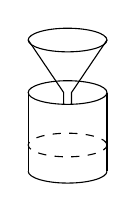
\begin{tikzpicture}
\pgfmathsetmacro{\h}{1}
\draw(0,0) circle (0.5cm and 0.15cm);
\draw ([shift={(180:0.5cm and 0.15cm)}]0,-\h) arc (180:360:0.5cm and 0.15cm);
\draw(-0.5,0)--++(0,-\h) (0.5,0)--++(0,-\h);
\draw[dashed] (0,-2/3*\h) circle (0.5cm and 0.15cm);
\draw(0,2/3*\h) circle (0.5cm and 0.15cm);
\draw(-0.5,2/3*\h)--(-0.05,0)--++(0,-0.15);
\draw(0.5,2/3*\h)--(0.05,0)--++(0,-0.15);
\end{tikzpicture}
\caption{مخروط چھلنی (سوال \حوالہ{سوال_تفرق_مخروط_چھلنی})}
\label{شکل_سوال_تفرق_مخروط_چھلنی}
\end{figure}
\انتہا{سوال}
%======================
\ابتدا{سوال}\ترچھا{اخراج قلب}
جرمنی کے اڈولف فک نے \سن{1860} کی دہائی میں دل سے گزرتے ہوئے خون کی  شرح ناپنے کا طریقہ ایجاد کیا جو آج بھی زیر استعمال ہے۔ اس وقت اس جملے کو پڑھتے ہوئے آپ کا دل تقریباً \عددی{\SI{7}{\litre\per\minute}} خون خارج کر رہا ہو گا جبکہ بالکل آرام سے بیٹھ کر \عددی{\SI{6}{\litre\per\minute}} اخراج متوقع ہے۔ بہت لمبی دوڑ لگانے والے کھلاڑی کا قلب  \عددی{\SI{30}{\litre\per\minute}} تک خون خارج کر سکتا ہے۔

قلب کے اخراج کا حساب
\begin{align*}
y=\frac{Q}{D}
\end{align*}
سے کیا جا سکتا ہے جہاں سانس سے خارج \عددی{\ce{CO2}} کی  ملی لٹر فی منٹ میں مقدار کو \عددی{Q} سے ظاہر کیا گیا ہے جبکہ پھیپھڑوں کو فراہم خون میں \عددی{\ce{CO2}} کی کثافت \عددی{\si{\milli\litre/\litre}} اور پھیپھڑوں سے خارج خون میں \عددی{\ce{CO2}} کی کثافت کے فرق کو \عددی{D} سے ظاہر کیا گیا ہے۔ یوں \عددی{Q=\SI{223}{\milli\litre/\minute}} اور \عددی{D=97-56=\SI{41}{\milli\litre/\litre}} کی صورت میں 
\begin{align*}
y=\frac{\SI{223}{\milli\litre/\minute}}{\SI{41}{\milli\litre/\litre}}\approx \SI{5.68}{\litre/\minute}
\end{align*}
ہو گا جو آرام سے بیٹھے شخص کے قلب کے اخراج کے کافی قریب ہے۔

فرض کریں کہ ہم جانتے ہیں کہ جب \عددی{Q=233} اور \عددی{D=41} ہوں تب \عددی{D} کی قیمت \عددی{2} اکائی فی منٹ سے گھٹ رہی ہے جبکہ \عددی{Q} میں کوئی تبدیلی نہیں پائی جاتی ہے۔قلب کے اخراج کو کیا ہو رہا ہے؟\\
جواب:\quad
\عددی{\tfrac{466}{1681}\,\si{\litre\per\minute}} سے بڑھ رہا ہے۔
\انتہا{سوال}
%====================
\ابتدا{سوال}\ترچھا{لاگت، آمدنی اور منافع۔}\quad
ایک ادارہ \عددی{x} اشیاء کو \عددی{c(x)} لاگت، \عددی{r(x)} آمدنی اور \عددی{p(x)=r(x)-c(x)} منافع کے ساتھ تیار کر سکتا ہے (تمام اعداد و شمار کو \عددی{1000} سے ضرب کریں)۔\عددی{x} اور \عددی{\tfrac{\dif x}{\dif t}} کی درج ذیل قیمتوں کے لئے \عددی{\tfrac{\dif c}{\dif t}}، \عددی{\tfrac{\dif r}{\dif t}} اور \عددی{\tfrac{\dif p}{\dif t}} کا حساب کریں۔ 
\begin{enumerate}[a.]
\item
\begin{align*}
r(x)=9x,\quad c(x)=x^3-6x^2+15x;\quad  \frac{\dif x}{\dif t}=0.1,\quad x=2
\end{align*}
\item
\begin{align*}
r(x)=70x,\quad c(x)=x63-6x62+\frac{45}{x};\quad \frac{\dif x}{\dif t}=0.05,\quad x=1.5
\end{align*}
\end{enumerate} 
\انتہا{سوال}
%==============
\ابتدا{سوال}\ترچھا{قطع مکافی پر حرکت۔}\quad
ایک ذرہ  قطع مکافی \عددی{y=x^2} پر ربع اول میں یوں حرکت کرتا ہے کہ اس کا \عددی{x} محدد \عددی{\SI{10}{\meter\per\second}} کی شرح سے بڑھتا جاتا ہے۔مبدا سے ذرہ تک خط، \عددی{x} محور کے ساتھ زاویہ \عددی{\theta} بناتا ہے۔ جب \عددی{x=\SI{3}{\meter}} ہو تب  \عددی{\theta} کس شرح سے تبدیل ہو گا؟\\
جواب:\quad
\عددی{\SI{1}{\radian\per\second}}
\انتہا{سوال}
%==========================
\ابتدا{سوال}\ترچھا{دوسرا قطع مکافی۔}\quad
ایک ذرہ دائیں سے بائیں جانب قطع مکافی \عددی{y=\sqrt{-x}} پر یوں  حرکت کرتا ہے کہ اس کا \عددی{x} محدد \عددی{\tfrac{8}{\meter\per\second}} سے گھٹتا ہے۔ مبدا سے ذرہ تک خط، \عددی{x} محور کے ساتھ زاویہ \عددی{\theta} بناتا ہے۔ جب \عددی{x=\SI{-4}{\meter}} ہو تب  \عددی{\theta} کس شرح سے تبدیل ہو گا؟
\انتہا{سوال}
%==========================
\ابتدا{سوال}\ترچھا{مستوی پر حرکت۔}\quad 
کارتیسی محدد پر حرکت کرتے ہوئے ذرہ کے  تعین گر \عددی{x} اور \عددی{y} محدد وقت \عددی{t} کے قابل تفرق تفاعل ہیں۔اگر \عددی{\tfrac{\dif x}{\dif t}=\SI{-1}{\meter\per\second}} اور \عددی{\tfrac{\dif y}{\dif t}=\SI{-5}{\meter\per\second}} ہوں تب مبدا سے ذرے کا فاصلہ کس شرح سے تبدیل ہو گا؟\\
جواب:\quad
\عددی{\SI{-5}{\meter\per\second}}
\انتہا{سوال}
%==========================
\ابتدا{سوال}\ترچھا{حرکت پذیر سایہ۔}\quad
\عددی{\SI{2}{\meter}} قد کا ایک شخص  گلی  میں روشنی کے کھمبے کی طرف \عددی{\SI{1.5}{\meter\per\second}} رفتار سے چل رہا ہے۔ کھمبے میں نسب بلب زمین سے \عددی{\SI{5}{\meter}} بلندی پر ہے۔جب شخص کھمبے سے \عددی{\SI{4}{\meter}} فاصلے پر ہو، اس کا سایہ کس شرح سے تبدیل ہو گا؟
\انتہا{سوال}
%=======================
\ابتدا{سوال}\شناخت{سوال_تفرق_گرتا_ہوا_گیند}\ترچھا{دوسرا حرکت کرتا سایہ۔}\quad
کھمبے پر بلب \عددی{\SI{15}{\meter}} بلندی پر نسب ہے۔کھمبے سے \عددی{\SI{10}{\meter}} فاصلے پر اتنی ہی بلندی سے ایک گیند کو زمین پر گرنے دیا جاتا ہے (شکل \حوالہ{شکل_سوال_تفرق_گرتا_ہوا_گیند})۔ آدھے سیکنڈ بعد زمین پر گیند کا سایہ کس رفتار سے حرکت کرے گا؟ (\عددی{g=\SI{9.8}{\meter\per\second\squared}})
\begin{figure}
\centering
\begin{minipage}{0.45\textwidth}
\centering
\begin{tikzpicture}[font=\small]
\draw[-latex](0,0)--(3.5,0)node[right]{$x$};
\draw(0,0)--(0,2)node[pos=0.5,left]{$\SI{15}{\meter}$}node[circ]{}node[left]{بلب};
\draw[name path=kslan](0,2)--(3,0)node[below]{$x(t)$}node[circ]{}node[above right]{سایہ};
\path[name path=kver](1,2)--(1,0);
\draw[name intersections={of={kslan and kver}}](1,2)node[ocirc]{}--(intersection-1)node[ocirc]{}node[pin=45:{\RL{آدھے سیکنڈ بعد}}]{};
\draw[dashed](intersection-1)--(1,0)node[below]{$10$};
\draw[-latex] (3,-0.5)--++(-0.5,0);
\end{tikzpicture}
\caption{گیند کا سایہ (سوال \حوالہ{سوال_تفرق_گرتا_ہوا_گیند})}
\label{شکل_سوال_تفرق_گرتا_ہوا_گیند}
\end{minipage}\hfill
\begin{minipage}{0.45\textwidth}
\centering
\begin{tikzpicture}[font=\small]
\pgfmathsetmacro{\ang}{atan(3/2)}
\draw(0,0)node[circ]{}node[below]{گاڑی}--++(3,0)--++(0,2)node[circ]{}node[right]{کیمرہ};
\draw(0,0)--(3,2);
\draw([shift={(-90:0.5)}]3,2) arc (-90:-90-\ang:0.5);
\draw(3,2)++(-90-\ang/2:0.8)node[]{$\theta$};
\draw(3,1)node[right]{$\SI{40}{\meter}$};
\RightAngle{(3,2)}{(3,0)}{(0,0)}
\draw[-latex](0,0.25)--++(0.25,0);
\end{tikzpicture}
\caption{گاڑی کی ویڈیو (سوال \حوالہ{سوال_تفرق_ویڈیو})}
\label{شکل_سوال_تفرق_ویڈیو}
\end{minipage}
\end{figure}
جواب:\quad
$\SI{490}{\meter\per\second}$
\انتہا{سوال}
%========================
\ابتدا{سوال}\شناخت{سوال_تفرق_ویڈیو}
آپ \عددی{\SI{80}{\kilo\meter\per\hour}} رفتار سے چلتی ہوئی  گاڑی سے \عددی{\SI{150}{\meter}} کے فاصلے پر  \عددی{\SI{40}{\meter}} کی بلندی سے گاڑی کی \ترچھا{ویڈیو}\حاشیہب{video} بنا رہے ہیں جو سیدھی آپ کی طرف آ رہی ہے (شکل \حوالہ{شکل_سوال_تفرق_ویڈیو})۔اس لمحے پر کیمرے کا زاویہ میلان سے شرح سے تبدیل ہو گا؟ دو سیکنڈ بعد یہ شرح کیا ہو گی؟  
\انتہا{سوال}
%==============================
\ابتدا{سوال}\ترچھا{برف کی پگھلتی تہہ۔}\quad
ایک لوہے کا کرہ جس کا رداس \عددی{\SI{0.1}{\meter}} ہے پر برف کی یکساں موٹائی کی تہہ جمائی جاتی ہے جو \عددی{\SI{10}{\centi\meter\cubed\per\second}} کی شرح سے پگھلتی ہے۔ جس لمحے پر  تہہ کو موٹائی \عددی{\SI{2}{\centi\meter}} ہو اس لمحے پر تہہ کی موٹائی کس شرح سے تبدیل ہو گی؟\\
جواب:\quad
$\tfrac{\dif r}{\dif t}=\SI{55}{\micro\meter\per\second}, \quad \tfrac{\dif S}{\dif t}=\SI{1.66}{\centi\meter\squared\per\second}$
\انتہا{سوال}
%============================
\ابتدا{سوال}\ترچھا{موٹروے پولیس۔}\quad
\عددی{\SI{1}{\kilo\meter}} بلندی پر ایک جہاز پشاور سے اسلام آباد کی موٹروے کے ٹھیک اوپر \عددی{\SI{500}{\kilo\meter\per\hour}} کی رفتار سے پرواز کرتے ہوئے موٹروے پر  سامنے سے آمد گاڑی کا فاصلہ \عددی{\SI{5}{\kilo\meter}} ناپتا ہے جو اس لمحے پر \عددی{\SI{100}{\kilo\meter\per\hour}} کی شرح سے گھٹ رہا ہے۔گاڑی کی رفتار تلاش کریں۔
\انتہا{سوال}
%============================
\ابتدا{سوال}\شناخت{سوال_تفرق_عمارت_سایہ}\ترچھا{عمارت کا سایہ۔}\quad
سال کے کسی ایک دن سورج \عددی{\SI{80}{\meter}} بلند عمارت کے ٹھیک اوپر سے گزرتا ہے (شکل \حوالہ{شکل_سوال_تفرق_عمارت_سایہ})۔ جب عمارت کا سایہ ہموار زمین پر \عددی{\SI{60}{\meter}} ہو، سایے کے سر سے سورج تک کا خط زمین کے ساتھ زاویہ \عددی{\theta} بناتا ہے جو اس لمحہ \عددی{0.27^{\circ}/\si{\minute}} کی شرح سے تبدیل ہوتا ہے۔ سایے کی لمبائی کس شرح سے گھٹتی ہے؟ جواب \عددی{\si{\centi\meter/\minute}} میں دیں اور ریڈیئن کا استعمال کرنا نہ بھولیں۔
\begin{figure}
\centering
\begin{tikzpicture}
\pgfmathsetmacro{\h}{1.5}
\pgfmathsetmacro{\ang}{60}
\pgfmathsetmacro{\len}{\h*tan(\ang)}
\draw(0,0) rectangle ++(0.5,1.5);
\draw(0,0.75)node[left]{$\SI{80}{\meter}$}node[above,rotate=-90]{عمارت};
\draw(0,0)--(\len+0.5,0)coordinate(kA)--++(150:4.5)node[circ]{}node[left]{سورج};
\draw([shift={(150:0.5)}]kA)  arc (150:180:0.5);
\draw(kA)++(150+15:0.8)node[]{$\theta$};
\end{tikzpicture}
\caption{عمارت کا سایہ (سوال \حوالہ{سوال_تفرق_عمارت_سایہ})}
\label{شکل_سوال_تفرق_عمارت_سایہ}
\end{figure}
جواب:\quad
$\SI{58.9}{\centi\meter/\minute}$
\انتہا{سوال}
%======================
\ابتدا{سوال}\ترچھا{چال قدمی۔}\quad
ایک چوراہے پر دو سڑک \عددی{90^{\circ}} زاویے سے آپس میں ملتے ہیں۔ایک سڑک پر عفت بریخنہ چوراہے کی جانب \عددی{\SI{2}{\meter\per\second}} کی رفتار سے بڑھتی ہے جبکہ دوسری سڑک پر اس کا چھوٹا بھائی زریاب خان \عددی{\SI{1.5}{\meter\per\second}} کی رفتار سے چوراہے سے دور چلا جاتا ہے۔جب عفت بریخنہ اور زریاب خان چوراہے سے بالترتیب \عددی{\SI{20}{\meter}} اور \عددی{\SI{15}{\meter}} کے فاصلے پر ہوں، زاویہ \عددی{\theta} کی شرح تبدیلی کیا ہو گی؟ 
\انتہا{سوال}
%======================
\ابتدا{سوال}\شناخت{سوال_تفرق_کھیل}\ترچھا{بچوں کا کھیل۔}
ایک کھیل میں کھلاڑی ابتدائی نقطہ الف سے دوڑ کر گھری کی الٹ رخ چکور راہ پر \عددی{\SI{6}{\meter\per\second}} کی رفتار سے چکر لگاتا ہے۔چکور کے اطراف کی لمبائی \عددی{\SI{30}{\meter}} ہے (شکل \حوالہ{شکل_سوال_تفرق_کھیل})۔
\begin{enumerate}[a.]
\item
جب کھلاڑی ابتدائی نقطہ الف سے \عددی{\SI{10}{\meter}} فاصلے پر ہو، اس کا نقطہ ج سے فاصلہ کس شرح سے تبدیل ہوتا ہے؟
\item
اس لمحے پر زاویہ \عددی{\theta_1} اور \عددی{\theta_2} کس شرح سے تبدیل ہوتے ہیں؟ 
\end{enumerate}
%
\begin{figure}
\centering
\begin{tikzpicture}
\draw(0,0)--++(0,2)node[pos=0.3333,circ]{}coordinate[pos=0.3333](kA)--++(-2,0)--++(0,-2)node[pos=0.5,left]{$\SI{30}{\meter}$}-++(2,0);
\draw(0,0)node[right]{الف};
\draw(0,2)node[right]{ب};
\draw(-2,2)node[left]{ج};
\draw(-2,0)node[left]{د};
\draw(-2,2)--(kA);
\draw([shift={(90:0.5)}]kA) arc (90:146.31:0.5);
\draw(kA)++(110:0.7)node[]{$\theta_2$};
\draw([shift={(0:0.5)}]-2,2) arc (0:-33.69:0.5);
\draw(-2,2)++(-15:0.7)node[]{$\theta_1$};
\end{tikzpicture}
\caption{بچوں کا کھیل (سوال \حوالہ{سوال_تفرق_کھیل})}
\label{شکل_سوال_تفرق_کھیل}
\end{figure}

جواب:\quad
(ا) \عددی{\tfrac{-12}{\sqrt{13}}\,\si{\meter\per\second}}، (ب) \عددی{\tfrac{\dif \theta_1}{\dif t}=\SI{-0.138}{\radian\per\second}}، \عددی{\tfrac{\dif \theta_2}{\dif t}=\SI{0.138}{\radian\per\second}}
\انتہا{سوال}
%=======================
\ابتدا{سوال}
ایک گھڑی کے سیکنڈوں کی سوئی کی لمبائی \عددی{\SI{20}{\centi\meter}} ہے۔جب یہ سوئی چار بجے پر ہو اس لمحہ بارہ بجے کی نشان سے اس کا فاصلہ کس شرح سے تبدیل ہو گا؟ 
\انتہا{سوال}
%============================
\ابتدا{سوال}\ترچھا{بحری جہاز۔}\quad
نقطہ \عددی{M} سے دو بحری جہاز آپس میں \عددی{120^{\circ}} کا زاویہ بناتے ہوئے روانہ ہوتے ہیں۔جہاز الف کی رفتار \عددی{\SI{28}{\kilo\meter\per\hour}} ہے جبکہ جہاز ب کی رفتار \عددی{\SI{20}{\kilo\meter\per\hour}} ہے۔ایک گھنٹہ بعد ان کے بیچ فاصلہ کس شرح سے تبدیل ہو گا؟\\
جواب:\quad
$4\sqrt{109}\,\si{\kilo\meter\per\hour}$
\انتہا{سوال}
%==========================
